\documentclass[12pt,a4paper,final]{article}
\usepackage[left=2.5cm,right=2.5cm,top=2.5cm,bottom=2.5cm]{geometry}

%% IDIOMA
\usepackage[utf8]{inputenc}
\usepackage[portuguese]{babel}

%% TRANSFORMAÇÕES ESTILO CSS
\usepackage{graphicx}

%% ESTÉTICA
\usepackage{enumerate}
\usepackage{booktabs}
\usepackage{amsmath, amsthm, amssymb, amsfonts}
\usepackage{multirow}
\usepackage[hyphens]{url}
\usepackage{subfig}

%% FONTE
\usepackage[T1]{fontenc}
%\usepackage[sc]{mathpazo} % Palatino with smallcaps
\usepackage{mathptmx}
\usepackage{eulervm} % Euler math

%% TIPOGRAFIA
\usepackage{parskip}
\usepackage[activate={true,nocompatibility},final,tracking=true,kerning=true,spacing=true,factor=1100,stretch=10,shrink=10]{microtype}

%% CODIGO
\usepackage{listings}
\usepackage{color}

\definecolor{dkgreen}{rgb}{0,0.6,0}
\definecolor{gray}{rgb}{0.5,0.5,0.5}
\definecolor{mauve}{rgb}{0.58,0,0.82}

\lstset{frame=tb,
  aboveskip=3mm,
  belowskip=3mm,
  showstringspaces=false,
  columns=flexible,
  basicstyle={\small\ttfamily},
  numbers=none,
  numberstyle=\tiny\color{gray},
  keywordstyle=\color{blue},
  commentstyle=\color{dkgreen},
  stringstyle=\color{mauve},
  breaklines=true,
  breakatwhitespace=true,
  tabsize=3
}

\title{Relatório 7 de TCC2/IC}
\author{Ly Sandro Amorim de Campos Salles\\Departamento de Física\\Universidade Federal do Paraná}
\date{\today}

\begin{document}
	\maketitle

  Desde o último encontro foram realizadas as seguintes atividades:

  A finalização do novo programa de simulações de autômatos celulares, disponível, com histórico de modificações, no endereço \url{https://github.com/Ly54ndr0/CellularAutomataExplorer}.

  Foi verificado que os algoritmos utilizados estão corretos e retornam valores corretos.

  Obtenção de cinco conjunto de dados, com 20000 pontos cada, para cada combinação de $q$ e $L$ com $q\in\{$ 
  $0.1,$ $0.2,$ $0.3,$ $0.4,$ $0.5,$ $0.6,$ $0.7,$ $0.8,$ $0.9,$
  $1,$ $1.2,$ $1.4,$ $1.6,$ $1.8,$ 
  $2,$ $2.2,$ $2.4,$ $2.6,$ $2.8,$ 
  $3,$ $3.2,$ $3.4,$ $3.6,$ $3.8,$
  $4,$ $4.2,$ $4.4,$ $4.6,$ $4.8,$
  $5,$ $5.2,$ $5.4,$ $5.6,$ $5.8,$
  $6,$ $6.2,$ $6.4,$ $6.6,$ $6.8,$
  $7,$ $7.2,$ $7.4,$ $7.6,$ $7.8,$
  $8,$ $8.2,$ $8.4,$ $8.6,$ $8.8,$
  $9,$ $9.2,$ $9.4,$ $9.6,$ $9.8,$ $10,$
  $11,$ $12,$ $13,$ $14,$ $15,$ $16,$ $17,$ $18,$ $19,$ $20,$
  $22,$ $24,$ $26,$ $28,$ $30,$ $32,$ $34,$ $36,$ $38,$ $40,$
  $42,$ $44,$ $46,$ $48,$ $50,$ $52,$ $54,$ $56,$ $58,$ $60,$
  $65,$ $70,$ $75,$ $80,$ $85,$ $90,$ $95,$ $100,$ $110,$
  $120,$ $130,$ $140,$ $150,$ $160,$ $170,$ $180,$ $190,$
  $200,$ $220,$ $240,$ $260,$ $280,$ $300,$ $320,$ $340,$ $360,$ $380,$
  $400,$ $420,$ $440,$ $460,$ $480,$ $500,$ $520,$ $540,$ $560,$ $580,$
  $600,$ $620,$ $640,$ $660,$ $680,$ $700,$ $720,$ $740,$ $760,$ $780,$
  $800,$ $820,$ $840,$ $860,$ $880,$ $900,$ $920,$ $940,$ $960,$ $980,$
  $1000\}$ e $L\in \{50, 100\}$.

  Foi consultado o ``Material de Estudos da Certificação CPA-10: Volume 4, Princípios de Investimento'', da Associação Brasileira das Entidades dos Mercados Financeiro e de Capitais (ANBIMA), o qual, entre outros assuntos, inclui a descrição de liquidez.
  
  Considerando que, no autômato do Stauffer, $q$ representa a velocidade máxima com que cada célula (que tem um estado que determina se ela está comprando ou vendendo) é capaz de mudar de estado; considerando a definição ``A liquidez de um ativo pode ser definida como a facilidade com que este ativo pode ser
  comprado ou vendido no mercado a um preço adequado. Em outras palavras, a liquidez indica
  justamente a velocidade com que um ativo pode ser negociado sem que a própria negociação
  influencie no preço do ativo.'' disponível na referência acima (ANBIMA); então definimos $q$ como Liquidez, a matriz como um mercado (conjunto de agentes que negociam um mesmo tipo de produto), as células dessa matriz como agentes mercadológicos, e o limiar (threshold) intrínseco a cada célula como um determinador do momento certo para vender ou comprar (considerando agentes que tomam decisões lógicas com base nas informações disponíveis). 

  Foi verificado que não ocorre a sopreposição da curva do potencial de Lennard-Jones no gráfico de afinidade em função de $q$, como ilustrado nas Figuras \ref{fig:L50} e \ref{fig:L100}.

  \begin{figure}[h]
    \centering
    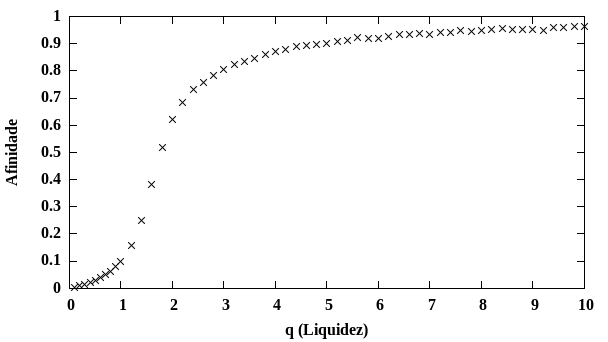
\includegraphics[width=.7\linewidth]{L50.png}
    \caption{Afinidade em função da liquidez para $L = 50$. A curva é uma sigmóide (como uma função logística), diferentemente do potencial de Lennard-Jones que se acreditava préviamente. À direita segue uma assíntota com limite igual a $1$ que foi verificada até $q=1000$.}
    \label{fig:L50}
  \end{figure}

  \begin{figure}[h]
    \centering
    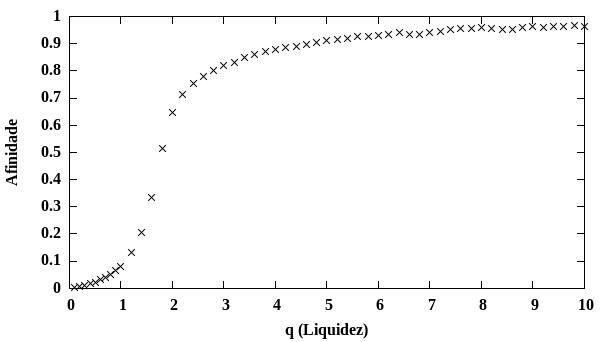
\includegraphics[width=.7\linewidth]{L100.png}
    \caption{Afinidade em função da liquidez para $L = 100$. Neste gráfico a derivada da curva tem um máximo maior do que para $L = 50$ para um maximizador próximo de $q = 2$.}
    \label{fig:L100}
  \end{figure}

  Foi escrito o seguinte protótipo de resumo:\\
  \textit{Utilizando um autômato celular bidimensional para simulações de compra e venda de agentes em um mercado, determinamos a intensidade com que esses agentes tendem a tomar decisões em conjunto, denominada afinidade, em função da liquidez do mercado. Essas simulações foram feitas para vários números diferentes de agentes. Descobrimos, nessa análise positiva, que a afinidade é uma função sigmóide da liquidez do mercado, variando um pouco com o número de agentes nesse mercado. Com base nesses gráficos percebemos que, para mercados com alta liquidez, como o de alimentos, a tendência a aglomeração de agentes é alta, o que explica as Centrais de Abastecimento CEASA. Analogamente, quando a liquidez do mercado é baixa, como no caso dos itens de colecionador e figurinhas de copa do mundo, a tendência de aglomeração é menor, fazendo com que existam mais aglomerados esparsamente distribuídos, como grupos de troca de figurinhas em várias praças de uma mesma cidade. Colateralmente foi desenvolvido um algoritmo de contagem de aglomerados para autômatos celulares em duas dimensões que se mostrou mais eficiente do que os utilizados atualmente.}\\ \textbf{Palavras-chave:} microeconomia, autômato celular, aglomeração, análise positiva, estocasticidade, modelagem, econofísica.

  Para os próximos dias, estas serão as tarefas realizadas:
  \begin{enumerate}
    \item Explicação do porquê de o limiar intrínseco a cada célula ser considerado como um determinador do momento certo para vender ou comprar;
    \item Finalização das simulações para $L = 250$ com os valores de $q$ listados acima;
    \item Simulação para as combinações com $L \in$ $\{ 500,$ $1000,$ $2000\}$ e $q\in\{$ 
    $0.2,$ $0.4,$ $0.6,$ $0.8,$ $1,$ 
    $1.2,$ $1.4,$ $1.6,$ $1.8,$ $2,$ 
    $2.2,$ $2.4,$ $2.6,$ $2.8,$ $3,$
    $3.2,$ $3.4,$ $3.6,$ $3.8,$ $4,$
    $4.2,$ $4.4,$ $4.6,$ $4.8,$ $5,$
    $5.2,$ $5.4,$ $5.6,$ $5.8,$ $6,$
    $6.2,$ $6.4,$ $6.6,$ $6.8,$ $7,$ 
    $7.2,$ $7.4,$ $7.6,$ $7.8,$ $8,$
    $8.2,$ $8.4,$ $8.6,$ $8.8,$ $9,$ 
    $9.2,$ $9.4,$ $9.6,$ $9.8,$ $10\}$, pois é nessa região que estão os dados que caracterizam a sigmóide;
		\item Leitura do artigo ``Stochastic Cellular Automata Model for Stock Market Dynamics'' dos autores M. Bartolozzi e A. W. Thomas;
		\item Pesquisa sobre como a volatilidade de mercado influencia na aglomeração dos agentes;
	\end{enumerate}

\end{document}
